Scalability fundamentally depends upon \textit{concurrent data structures}, structures that can be used by many threads simultaneously with performance scaling linearly with the number of threads.  Concurrent data structures are a well-studied topic and concurrent versions of most popular serial data structures have been discovered\cite{HSBook}.  Concurrency libraries even exist for some high level programming languages like Java.\cite{JavaUtilConcurrent}  But implementing concurrent data structures in systems languages without garbage collectors is a problem unto itself, even though such languages are demanded by high performance programmers.

High performance code is coveted in a number of fields including scientific computing, computer games, machine learning, and more.  Such code is written in languages that are \textit{close to the machine}, with data types and operations that intuitively and directly correspond to hardware primitives.\cite{Ritchie}  They permit programmers to select a data layout and alignment that optimizes cache usage, omit safety instructions (such as bounds-checking), and eschew generic types that tend to add levels of indirection.  By sacrificing these kinds of abstractions favored by higher level languages, they permit programmers to tune code and maximize performance, particularly on a single core.

As applied to serial data structures, this is the bread-and-butter of low-level languages like C, and it's why other languages write interface guidelines for programmers to hook C modules into their applications.  As applied to concurrent data structures, however, C provides little programmer support.

The core correctness problem is one of reclaiming memory from nodes visible to multiple threads.  Two threads access a node, one reading and the other removing, and the two must agree on a protocol to ensure the data the reader accesses is valid for as long as it holds a reference.  This complexity is papered over when concurrent data structures are introduced into the literature.\cite{ShavitLotanQueue, LindenPriority, HashTables, Harris}

As presented, these structures ``just work'' in garbage collected languages since the remover is safely able to drop the reference to the removed node.  But although C has good, sturdy conservative garbage collectors,\cite{BDW, DotNetGC} high performance applications tend to avoid them because of unpredictable delays and low scalability as compared with the multitude of other techniques C programmers apply to meet this challenge.  These techniques tend to be tailored to each structure and require invasive modification of the operations or place restrictions on where pointers are allowed to be stored and how/when they can be dereferenced.\cite{HP, DTA, StackTrack, Threadscan, RCU, RLU}

This involves a reinvention of the wheel of memory reclamation for every data structure in every concurrent application or library.  Worse, in a library setting, few techniques restrict themselves to the implementation of the data structure, itself.  Code that uses these libraries needs to know about the reclamation technique being employed if they ever hold pointers directly to data structure internal memory.  Between a conscious rejection of garbage collectors and the development of these alternatives, C provides a good case study in the present trade-off between performance, and code simplicity and modularity.  In academic papers and micro-benchmarks, the memory is typically just permitted to leak.

Rust makes a foray into this excluded domain with compiler-based proofs that statically determine when most memory can be deallocated.\cite{Rust}  When this is impossible, as in a concurrent data structure, Rust has tools such as \textit{reference counting} that can be employed to detect unreachable memory, but this has limited applicability.  Reference counting is slow as applied to structures that do extensive traversing (by adding a write to every read).  This performs well enough for hash table-based dictionaries and some other common structures, but it thrashes the cache in structures with nodes that tend to get touched frequently such as lists, trees, etc.  Further, it's altogether non-applicable to structures with cycles, since nodes removed from, e.g., a graph, may hold references to one another, and though they may all be unreachable, none can be deallocated.  Last, hooking a Rust-implemented concurrency library into another language is made difficult by the fact that the other language needs to know about the reference counters, rendering the libraries non-modular.

Languages like C and Rust are good at what they do, but they aren't designed for implementing concurrent data structures.  The space we've defined for such a language is expressed by the following criteria:

\begin{enumerate}
        \item \textbf{Close to the Machine:} Achieve high performance on a single core, competitive with C.
        \item \textbf{Modular:} Facilitate development of concurrent data structures that expose only their interfaces to callers.
        \item \textbf{Compatible:} Work as a drop-in replacement for C when inter-operating with other programming languages including C, itself.
\end{enumerate}

In this work we introduce DEF, a language designed to integrate seamlessly into C, that provides support for high performance, concurrency programming.  Seamless integration (as in fig.~\ref{fig:seemless-integration}) means that DEF understands C types, data structures, variables, and function declarations and can read them from C header files; and that a C header file can be automatically generated from a DEF source file, allowing C to interface with anything exported from DEF.  By virtue of this, DEF obtains the ability to inter-operate with other programming languages that have C hooks.

\begin{figure}[htbp!]
        \centering
        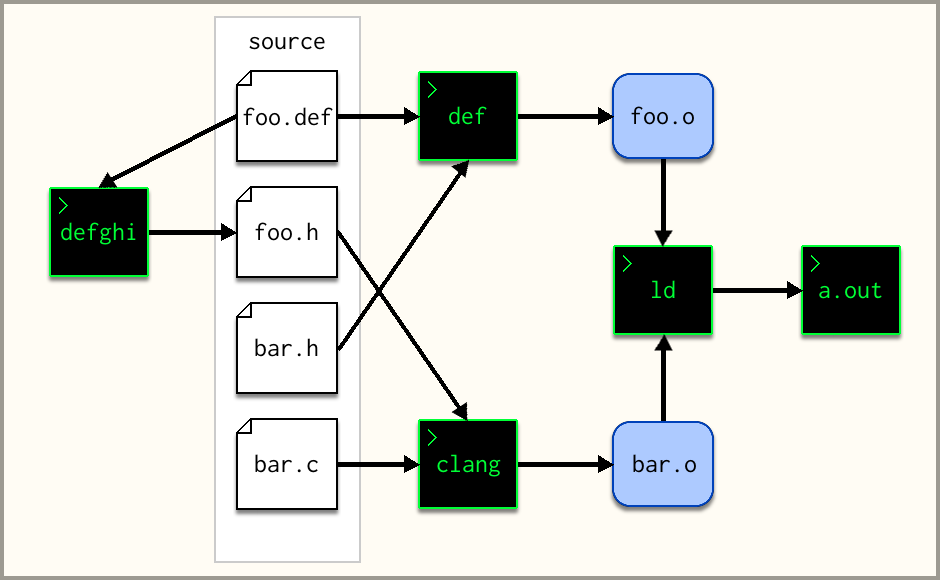
\includegraphics[scale=0.25]{gfx/seemless-integration}
        \caption{Integration between DEF and C source code can be done seamlessly by generating a C header file from the DEF source file, using the \texttt{defghi} utility, and importing/including the necessary header files into the respective source files.  Objects can be linked together as usual.}
        \label{fig:seemless-integration}
\end{figure}

DEF provides primitives for traditional low-level memory management in the form of \texttt{new} and \texttt{delete}, but also adds a \texttt{retire} keyword for use with pointers that may be visible to multiple threads.  The expectation is that memory can be allocated and deallocated, just as it is in normal C programs, and \texttt{new} and \texttt{delete} can be configured to use an application-specific allocator, since performance engineers generally look for the allocator that performs best on their application.  But when memory is shared in a concurrent data structure, \textit{invisible readers}, threads that perform nothing but read operations on a node (and are, therefore, invisible to a thread that might want to free it), memory can be retired and tracked by a special-purpose runtime.

The rationale is that no tracking needs to take place on most memory in an application, and that the programmer has a good sense of when memory can \textit{probably} be deallocated (e.g., when a node is removed from the structure).  \texttt{retire} is a notification the programmer provides to the compiler that a pointer should now be tracked.  In contrast to a garbage collector, that tracks and traces all memory it allocates, \texttt{retire} allows DEF to provide a more streamlined approach.

\texttt{retire}, moreover, represents the idea of \textit{automatic on-demand} memory reclamation as a part of concurrent data structure design.  It's tempting to argue that conventional designs are agnostic to memory reclamation, but to programmers, they represent the leaky or garbage collected models.  Any other model requires modification of the data structure or the functions that access it.  Automatic on-demand is typically a one-liner addition placed where \texttt{free} would be in a serial data structure.

Regarding legacy C compatibility, DEF's native runtimes are the C runtime library and those that are required for support for concurrency (Forkscan\cite{Forkscan}) and parallelism (Cilk\cite{BlumofeCilk}), insofar as they are actually used in the program.  Adding DEF to an existing application, therefore, creates no additional runtime burden or potential dependency conflicts.

As proof of concept, we implemented a benchmark suite including various concurrent data structures in DEF with corresponding implementations in C.  Since C benchmarks often forgo memory reclamation altogether, or reuse memory based on knowledge of the benchmark usage patterns,\cite{Synchrobench, Scal} the C implementations in our benchmark are leaky.

DEF demonstrates competitive performance with C on a single core (as shown in the benchmark results), doesn't require applications to know anything about data structure implementation, and interfaces with C simply and intuitively.
